\documentclass{beamer}% тип документа
% далее идёт преамбула
\usepackage{blindtext}
\usepackage{hypcap}
\usepackage[T2A,T1]{fontenc}
\usepackage[utf8]{inputenc}
\usepackage[russian]{babel}
\usepackage{graphicx}
\usepackage{datetime}
\usepackage{multicol}



\usepackage{caption}
\captionsetup[figure]{font=scriptsize,labelfont=scriptsize}

\begin{document}% начало презентации

\title{Разработка стохастической модели роста филамента в структуре оксидной пленки}
\author{Соловьёв Максим Андреевич}
\date{\today}
\institute{Кафедра физики твердого тела,
Физический факультет,\\
Московский государственный университет имени М.В.Ломоносовва.\\
Научный руководитель: кандидат физико-математических наук\\
    Бажанов Дмитрий Игоревич}



\begin{frame}% первый слайд
\begin{figure}
    \centering
    
\includegraphics[width=60px]{img/ff-sign.png}
\end{figure}
\maketitle
\end{frame}

\begin{frame}{Мемристор}
\begin{multicols}{2}
Мемристор - это пассивный элемент в микроэлектронике, способный изменять свое сопротивление в зависимости от протекающего через него заряда. 
\footnotetext[1]{
    Journal of Vacuum Science and Technology B 29, 01AD03 (2011); doi: 10.1116/1.3521503
}
\begin{figure}
    \centering
    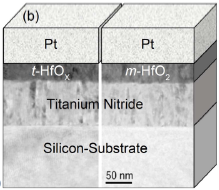
\includegraphics[width=85px]{img/real_memristor.PNG}
    \caption{Пример устройства реального мемристора%
\footnotemark[1]
}
\end{figure}
\columnbreak
    \begin{figure}
        \centering
        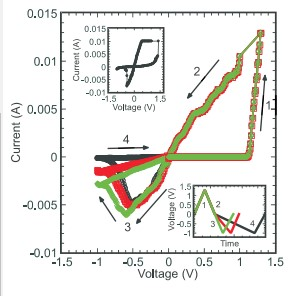
\includegraphics[width=150px]{img/vac_memrister.jpg}
        \caption{ВАХ реального мемристора%
    \footnotemark[1]
    }
    \end{figure}
\end {multicols}
% \footnotetext[2]{G. C. Jegert, “Modeling of Leakage Currents in High-k Dielectrics,” Ph.D. Dissertation, Tech. Univ. Munich,
% Germany, December 2011. }
\end{frame}

\begin{frame}{Мотивация}
\begin{multicols}{2}

% Мемристор может быть использован как синапс в нейроморфных сетях.

% Нейроморфные сети, имеют большой потенциал, так как крайне производительны по сравнению с традиционными реализациями нейронных сетей.

% Соответственно, моделирование мемристоров для определения разных их свойств - значимая область исследования.

Мемристор может быть использован как синапс в нейроморфных сетях.
Соответственно, моделирование разных свойств мемристора имеет большой потенциал.
\columnbreak
    
    \begin{figure}
        \centering
        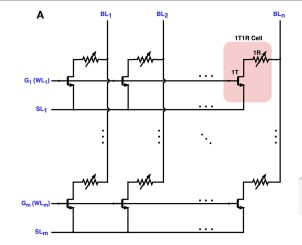
\includegraphics[width=160px]{img/sinaps-memristor-scheme.jpg}
        \caption{Принципиальная схема использования мемристора как синопса в нейроморфной сети%
        \footnotemark[2]
    }
    \end{figure}
    \footnotetext[2]{%
        Guo* Y, Wu H, Gao B and Qian H(2019) Unsupervised Learning on Resistive Memory Array Based Spiking Neural Networks. Front. Neurosci. 13:812. doi: 10.3389/fnins.2019.00812
        }%
\end{multicols}

\end{frame}


%Цель работы - что собираюсь делать и как моделировать
\begin{frame}{Цель работы}

Создание симулятора, позволяющего моделировать мемристор
и протекающие в нем процессы.
\begin{figure}
    \centering
    \includegraphics[width=300px]{schemes/model/model.pdf}
    \caption{
        Принципиальная схема симулятора
}
\end{figure}






\end{frame}

\begin{frame} {Симулируемая структура}
    \begin{itemize}
        \item Структура мемристора - слой диэлектрика, заключенный между парой электродов.
        \item Проводимость мемристора определяется ростом в нем определенной структуры - филаменты (нити).
        \item Филамент в большинстве случаев формируется на неоднородности электрода, поэтому неоднородность добавлена к электроду. \footnotemark[3]
    \end{itemize}

    \begin {multicols} {2}
    \begin{figure}
        \centering
        \includegraphics[height=80px]{schemes/simulator/simulator.pdf}
        %\vspace {11px}
        \caption {Симулируемая структура}
    \end{figure}
    
    \columnbreak

    \begin{figure}
        \centering
        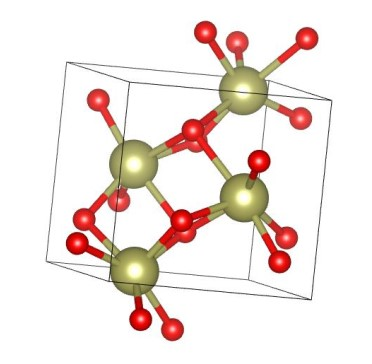
\includegraphics[height=80px]{img/POSCAR.jpg}
        \vspace {12px}
        \caption {Моноклинный \(HfO_2\)}
    \end{figure}

\end{multicols}

\footnotetext[3]{J. Appl. Phys. 125, 234503 (2019); https://doi.org/10.1063/1.5094864}

\end{frame}

\begin{frame} {Реакции}

    \begin {multicols} {2}

    \textbf{Ионные реакции}
    \begin {multicols} {2}
    \begin{figure}
        
        \centering
        \includegraphics[width=60px]{schemes/reacts/R1.pdf}
        \caption{Образование пары ион-вакансия}
        
    \end{figure}

    \columnbreak
    \begin{figure}

        \centering
        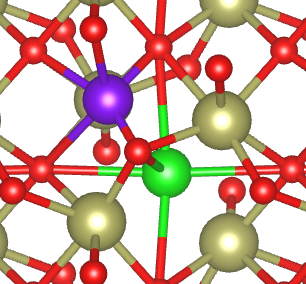
\includegraphics[width=60px]{schemes/reacts/R3.pdf}
        \caption{Рекомбинация пары ион-вакансия}

    \end{figure}

    \end{multicols}

    \begin {multicols} {2}
        
    \begin{figure}

        \centering
        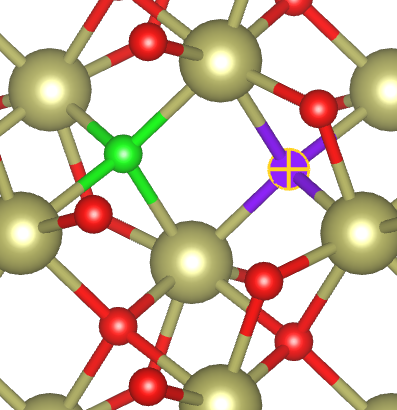
\includegraphics[width=60px]{schemes/reacts/R2.pdf}
        \caption{Перескок иона кисловода между межузельными положениями}

    \end{figure}
    \columnbreak
    \begin{figure}

        \centering
        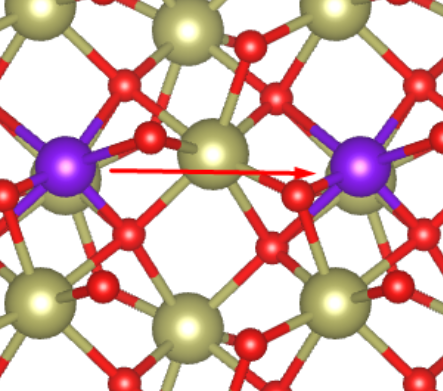
\includegraphics[width=60px]{schemes/reacts/R4.pdf}
        \caption{Перескок иона кислорода мижду узловыми положениями}

    \end{figure}
    \end{multicols}

    \columnbreak

    \textbf{Электронный транспорт и динамика}
    \begin{itemize}
        \item Эффект Шотки
        \item Эмиссия Пуля-Френкеля
        % \item Прямое туннелирование
        % \item Эффект фовлера Нордхелма
        \item Туннелирование с помощью ловушек (TAT)
    \end{itemize}

    \end{multicols}
\end{frame}

%Слайд с ионными реакциями
% \begin{frame}{Ионные реакции}
%     \begin{figure}

%         \centering
%         \includegraphics[height=40px]{schemes/reacts/types.pdf}

%     \end{figure}




% \end{frame}

% %Слайд для описания электронных реакций
% \begin{frame}{Электронные реакции}



% \end{frame}

%Слайд для формул, описывающих разные ракции

\begin{frame}{Математические основы модели} {Кинетический метод Монте-Карло}

%\textbf{Кинетический метод Монте-Карло}


В системе заданы N реакций с частотами: $\nu_i$.\
За каждый КМК шаг выбирается 1 реакция:
\[S_i = \sum_{j=1}^{i}{\nu_j}\]
\[R \in U[0,S_N)\]
\[S_i \le R < S_{i+1}\] 

\begin{figure}
    \centering
    \includegraphics[width=150px]{schemes/KMK_math/kmk_math.pdf}
\end{figure}

$\tau = \frac{1}{S_N}$ - время, за которое происходит этот шаг КМК.

\end{frame}

% Для ионных реакций:

\begin{frame}{Математические основы модели} {Частоты реакций}


    \begin {scriptsize}
    \begin {multicols} {2}

    Напряжение находится как:

    \[U = \frac{l\cdot U_{cond}}{D}+U_{evald}\],

    Частоты протекания ионных реакций находятся по формуле:

    \[\nu_{ion} = \nu _0 \cdot
    \exp{\left(-\frac{E_r-\gamma \Delta q \Delta U}{k_bT}\right)} \cdot
    %\exp{(-\frac{2\Delta r}{a})}
    \],

    Частоты перескока между ловушек:
    
    \[\nu_{tat} = \nu _0 \cdot
    \exp{\left(-\frac{E_r- e \Delta U}{k_bT}\right)} \cdot
    \exp{\left(-\frac{2\Delta r}{\xi}\right)}
    \]

    \columnbreak
    
    \textbf{Параметры}

    \(\nu_o = 10^{13} s^{-1} \)
    %\footnotemark[4] \footnotetext[4] {https://doi.org/10.1016/j.microrel.2017.12.021}

    \(\gamma = 4.0  \) 
    \footnotemark[4] \footnotetext[4]{Appl. Phys. Lett. 82, 781 (2003); https://doi.org/10.1063/1.1541096} 

    \(\xi = 2 \text{\r{A}}\) 
    %\footnotemark[5] \footnotetext[5]{Phys. Rev. Lett. 93, 177206 – Published 22 October 2004} 
    \hspace{10px}
    \begin{tabular}{|l|l|}
          Реакция & Барьер (эВ) \\ 
          R1 &  \(6.4\) \\
          R2 &  \(1.4\) \\
          R3 &  \(2.3\) \\
          R4 &  \(4.1\) \\
        TAT &  \(0.2-0.4\) 
        \footnotemark[5] \footnotetext[5]{Appl. Phys. Lett. 89, 042904 (2006); https://doi.org/10.1063/1.2234840}
        \end{tabular}


        \begin{figure}
            \centering
            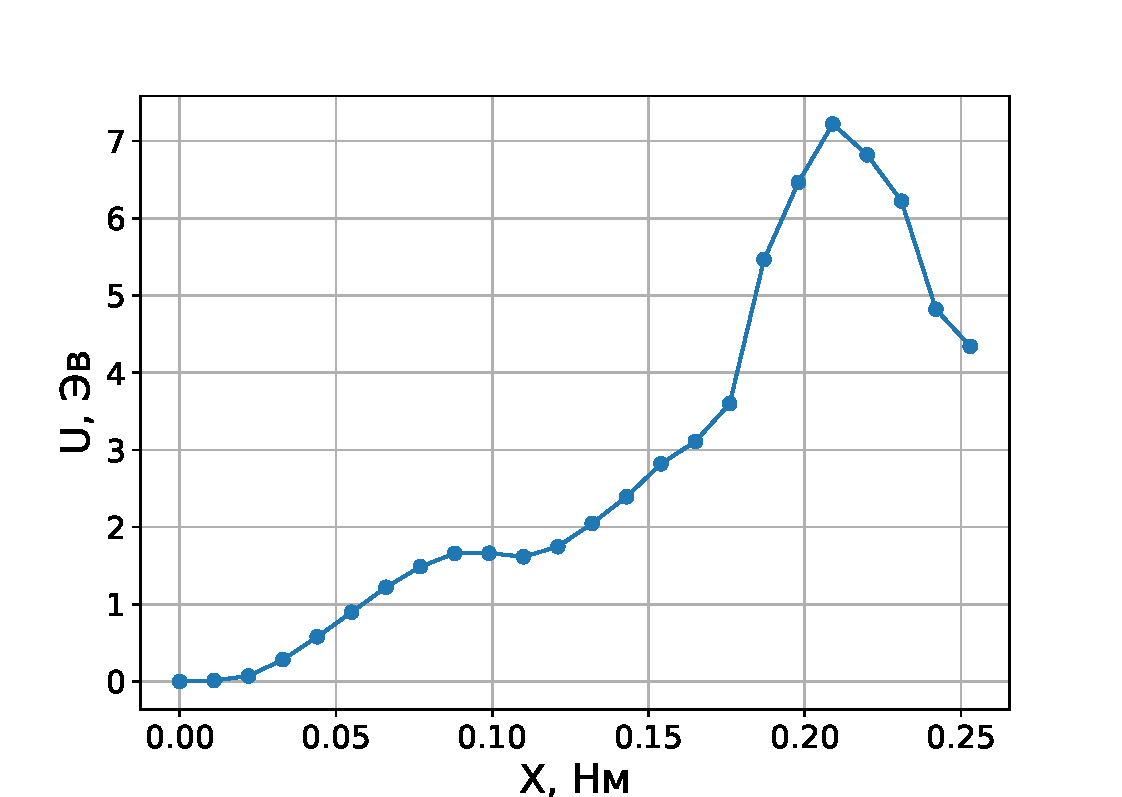
\includegraphics[width=90px]{img/R1_exexexe.pdf}
            \hspace{20px}
            \caption{DFT расчет для барьера реакции R1}
        \end{figure}


    \end {multicols}

    \end {scriptsize}

\end{frame}

\begin {frame} {Ток}

\begin {footnotesize}

\begin {multicols} {2}
Для нахождения тока, протекающего через мемристор учитываются определенные механизмы течения тока:

\[I_{ion} = \sum_{i=1}^{N_{ion}} \frac{\Delta q_{i} \Delta r_i} {D \tau } \]

\[I_{tat} = \sum_{i=1}^{N_{tat}} \frac{\Delta q_{i} \Delta r_i} {D \tau } \]

\columnbreak

$I_{shottky} =  \int  {j_{shottky}dV}$

$I_{pf} = \int {j_{pf}dV}$

\hspace{30px}

\textbf{Параметры}

$E_b = 0.9$ Эв \footnotemark[8]

$\Phi = 3.5$ Эв

$\epsilon_{opt} = 4.0$ \footnotemark[6]

$\rho_0 = 1.7 \cdot 10^{14} \text{см}^{-3} $ \footnotemark[6]

$\mu = 10^-3 \frac{\text{см}}{\text{В}\cdot\text{с}} $


\end{multicols}
$
    j_{shottky} = \frac{e m k_b^2 T^2} {2 \pi^2 \hbar^3}
    \exp\left[-\frac{1}{k_b T}\left(E_b-\sqrt{\frac{e^3 F}{4\pi\epsilon_0\epsilon_{opt}}}\right)\right]
$ 
\footnotemark[6]\footnotetext[6]{Popescu, Dan Horia. Modeling of Leakage Currents in High-k Dielectrics for Future DRAM Application. Diss. Technische Universität München, 2015.}

$
    j_{pf} = e\mu\rho_0 F \exp 
    \left[-\frac{1}{k_bT}\left(\Phi-\sqrt{\frac{e^3 F}{4\pi\epsilon_0\epsilon_{opt}}}\right)\right]
$
\footnotemark[7]\footnotetext[7]{ Basic Solid State Physics. V. 239, 59-70 (2003);
https://doi.org/10.1002/pssb.200303239}

% $
%     j_{direct} = 
% $

\end {footnotesize}

\footnotetext[8]{Journal of Vacuum Science \& Technology B 31, 01A105 (2013); https://doi.org/10.1116/1.4767125}

\end{frame}


%Используемые в модели константы
% \begin{frame}{Параметры и константы}
%     \begin{table}
%         \begin{tabular}{llc}
%           Параметр & Величина\\ 
%           Базовая частота (\(\nu _0\)) &
%           \(10^{-13} s^{-1}\) \\
%           \(\gamma\) & 4.0 \footnotemark[4]\\
%         \end{tabular}
%         \caption{Базовые константы}
%       \end{table}

%       \begin{table}
%         \begin{tabular}{llc}
%           Реакция & Барьер (эВ) \\ 
%           R1 &  \(6.4\) \\
%           R2 &  \(1.4\) \\
%           R3 &  \(0.8\) \\
%           R4 &  \(4.1\) \\
%           E1 &  \(0.3\) \\
%           E2 &  \(0.3\) \\
%           E3 &  \(0.3\) \\
%         \end{tabular}
%         \caption{Барьеры реакций}
%       \end{table}

%       \footnotetext[4]{Appl. Phys. Lett. 82, 781 (2003); https://doi.org/10.1063/1.1541096}
% \end{frame}

% \begin{frame} {Найденные барьеры}

%     \begin {multicols}

%     \begin{figure}

%         \centering
%         \includegraphics[width=100px]{img/barrier/R1}
%         \caption{Барьер R1}

%     \end{figure}

%     \begin{figure}

%         \centering
%         \includegraphics[width=100px]{img/barrier/R1}
%         \caption{Барьер R2}

%     \end{figure}
%     \columndreak

%     \begin{figure}

%         \centering
%         \includegraphics[width=100px]{img/barrier/R1}
%         \caption{Барьер R3}

%     \end{figure}

%     \begin{figure}

%         \centering
%         \includegraphics[width=100px]{img/barrier/R1}
%         \caption{Барьер R4}

%     \end{figure}
%     \end{multicols}
    
% \end{frame}

%Слайд с видом всей смоделированной структуры

% \begin{frame}{Смоделированная структура}
%     \begin{figure}
%         \centering
%         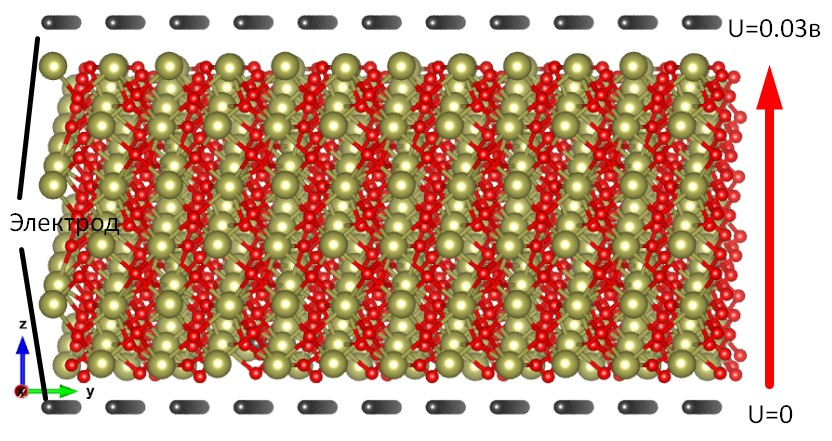
\includegraphics[width=300px]{img/model-result-v3.jpg}
%     \end{figure}

% \end{frame}

%На этом слайде будут/ет картинка с полученным филаментом.
\begin{frame}{Смоделированная структура}{}

В результате работы удалось смоделировать рост филамента в мемристоре.

\begin {multicols} {2}

\begin{figure}
    \centering
    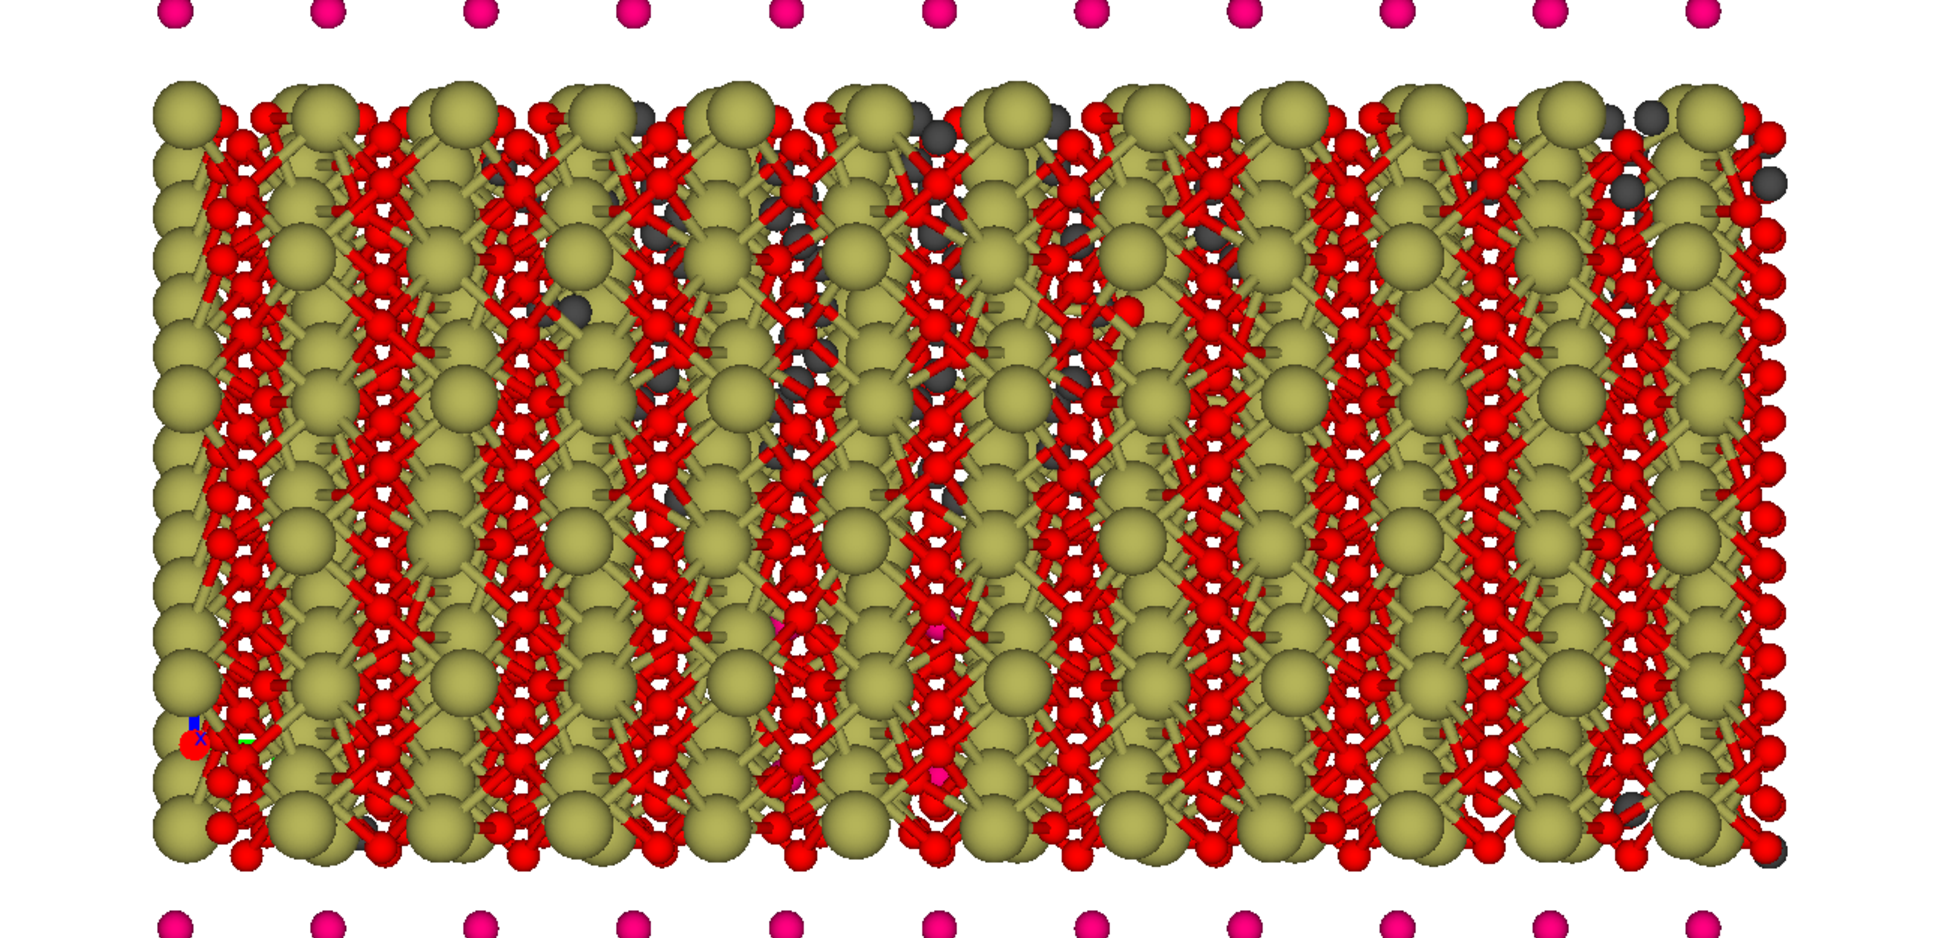
\includegraphics[height=60px]{img/11000_full_ex.pdf}
    \caption{Полная смоделированная структура.
    }
\end{figure}
\columnbreak

\begin{figure}
    \centering
    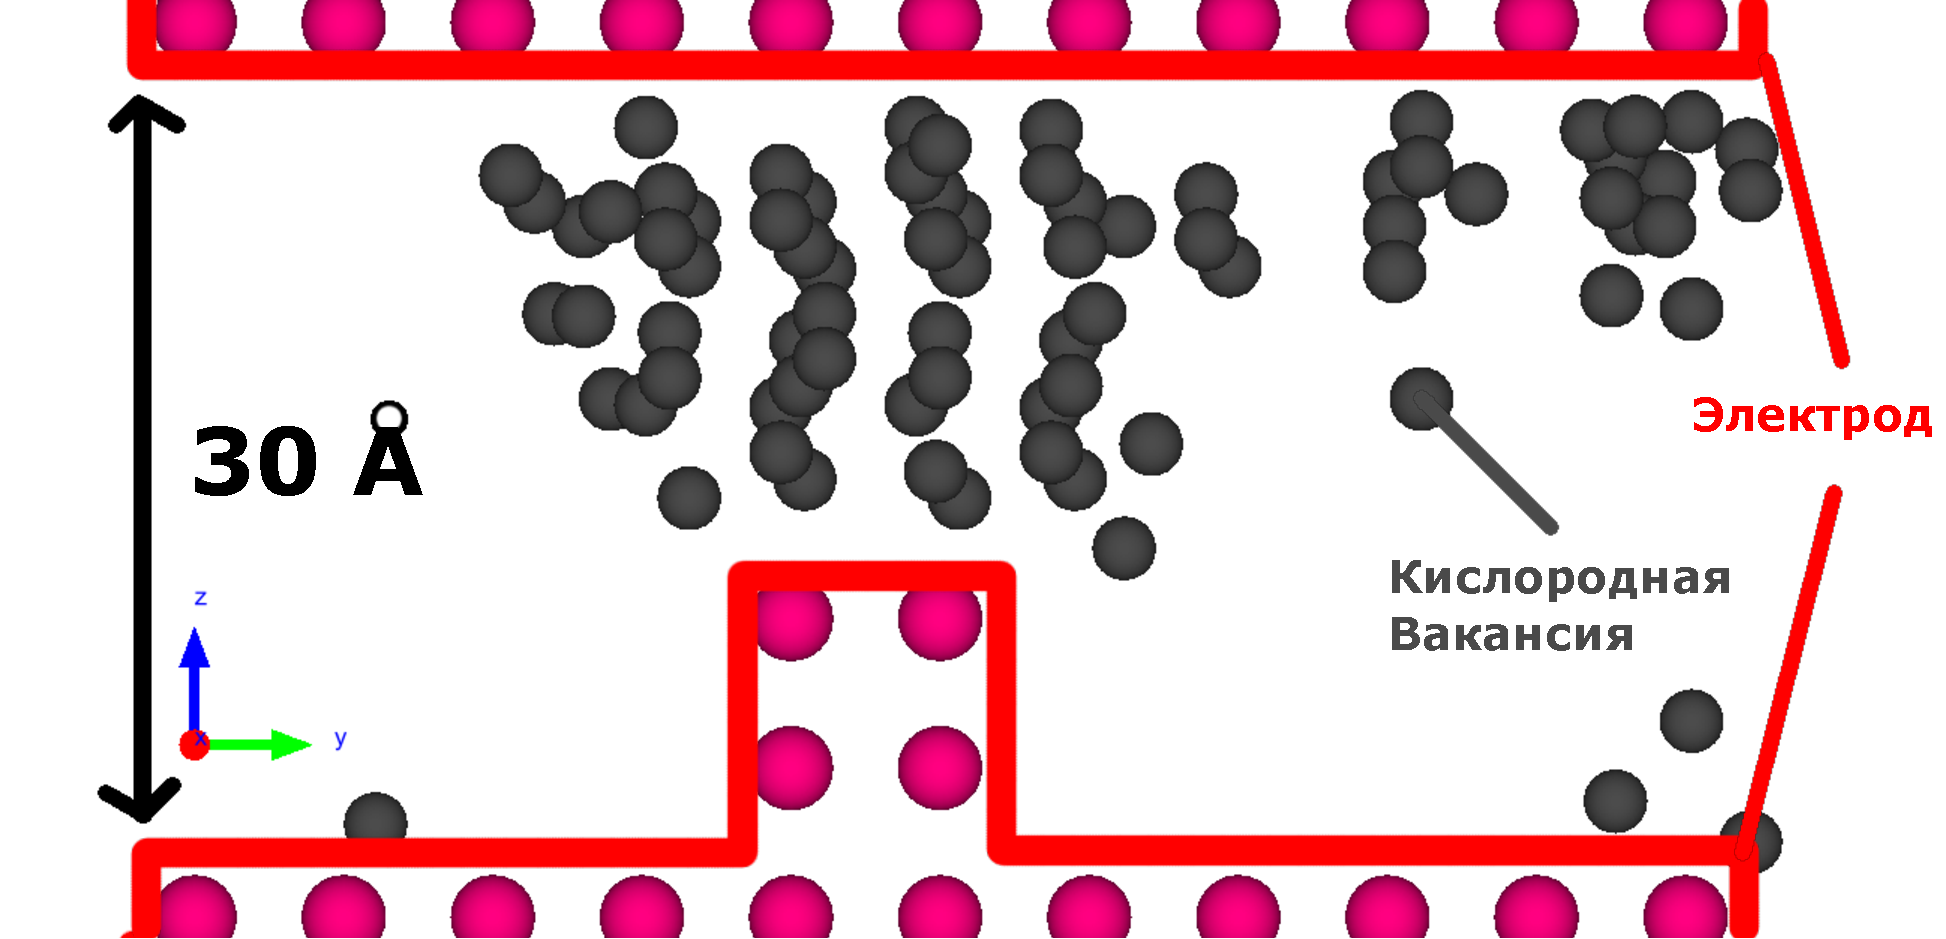
\includegraphics[height=60px]{img/11000_ex.pdf}
    \caption{Филамент в мемристоре при напряжении 0.9В между электродами.
    }
\end{figure}

\end{multicols}

\begin {multicols} {3}

\begin{figure}
    \centering
    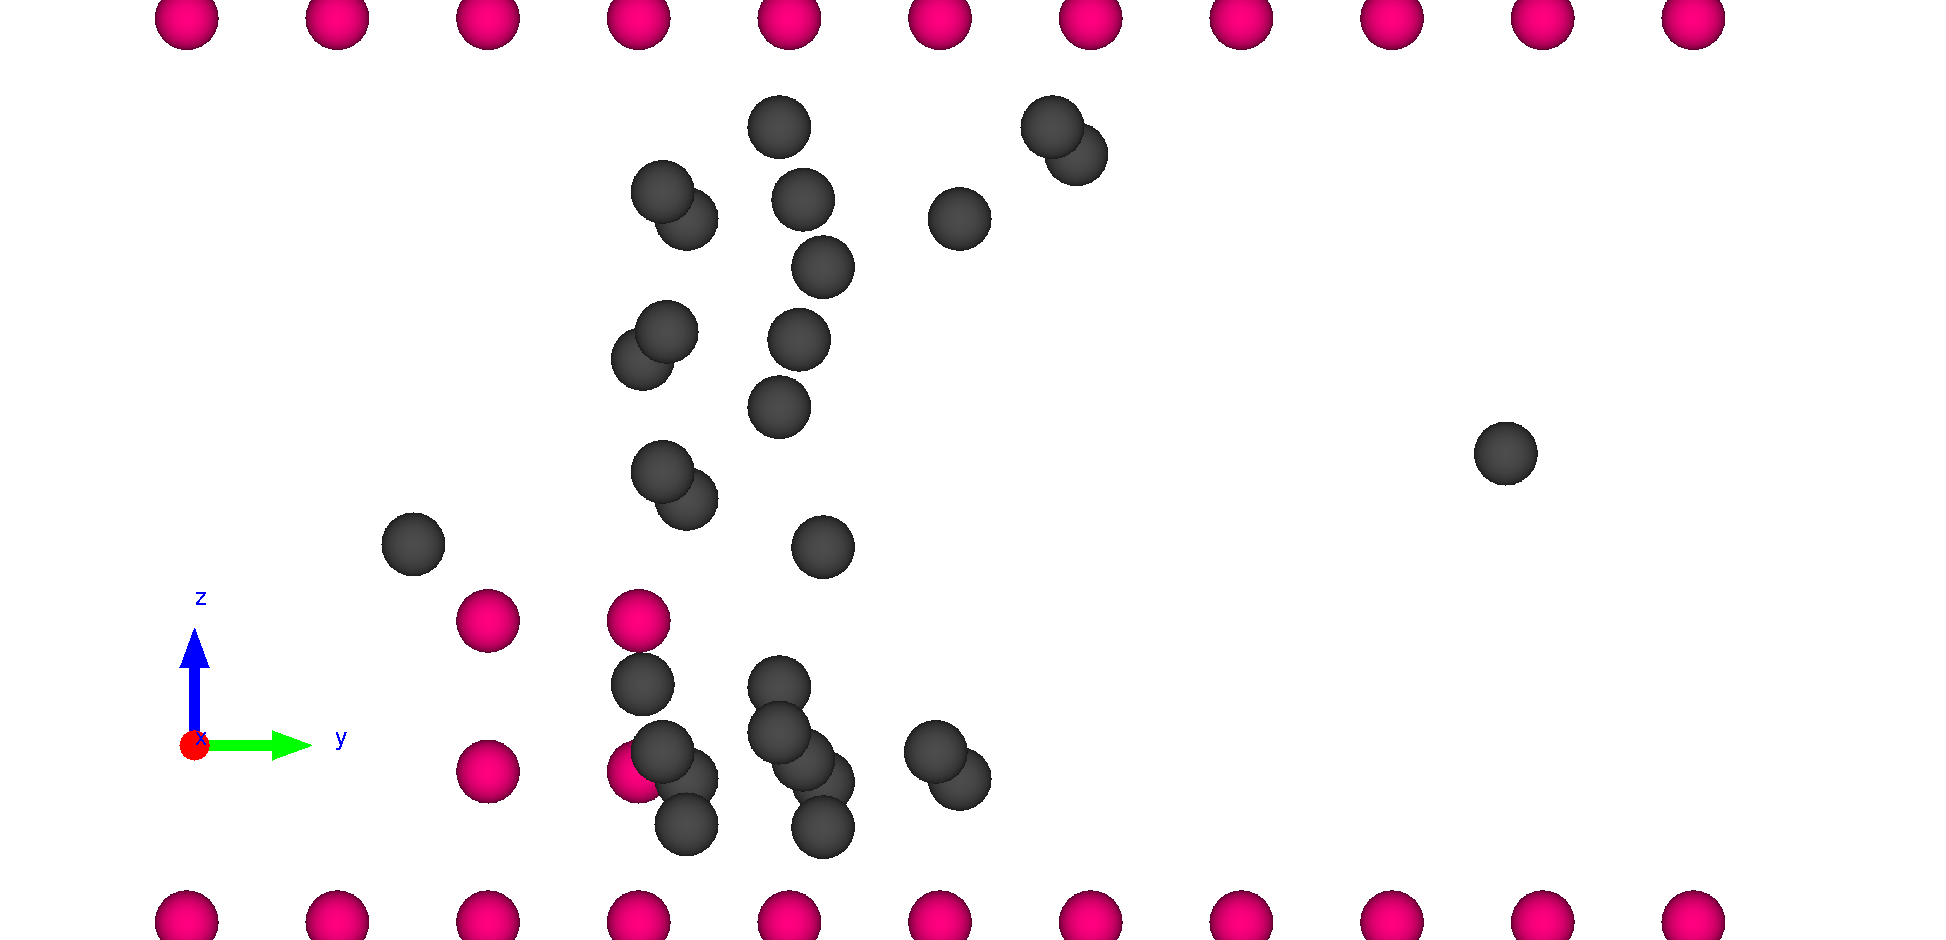
\includegraphics[height=50px]{img/80.pdf}
    \caption{Разрушение филамента в процессе RESET после 800 шагов КМК
    }
\end{figure}

\begin{figure}
    \centering
    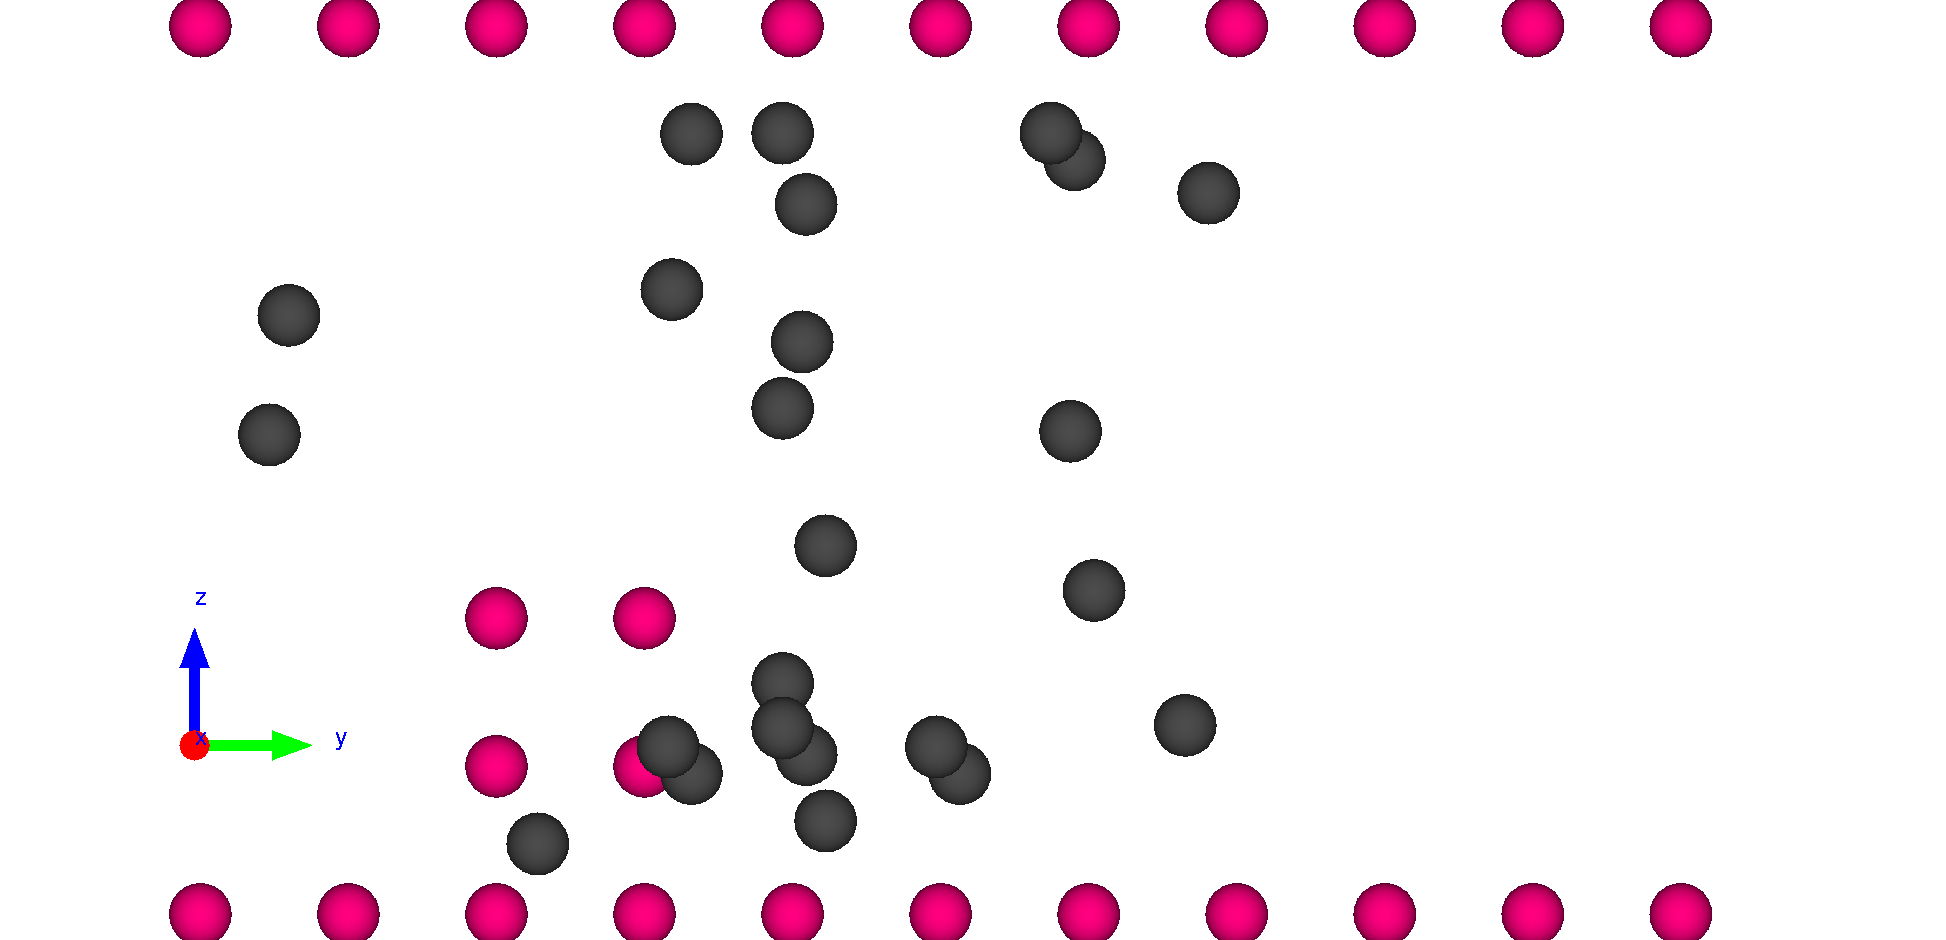
\includegraphics[height=50px]{img/150.pdf}
    \caption{Разрушение филамента в процессе RESET после 1500 шагов КМК
    }
\end{figure}

\begin{figure}
    \centering
    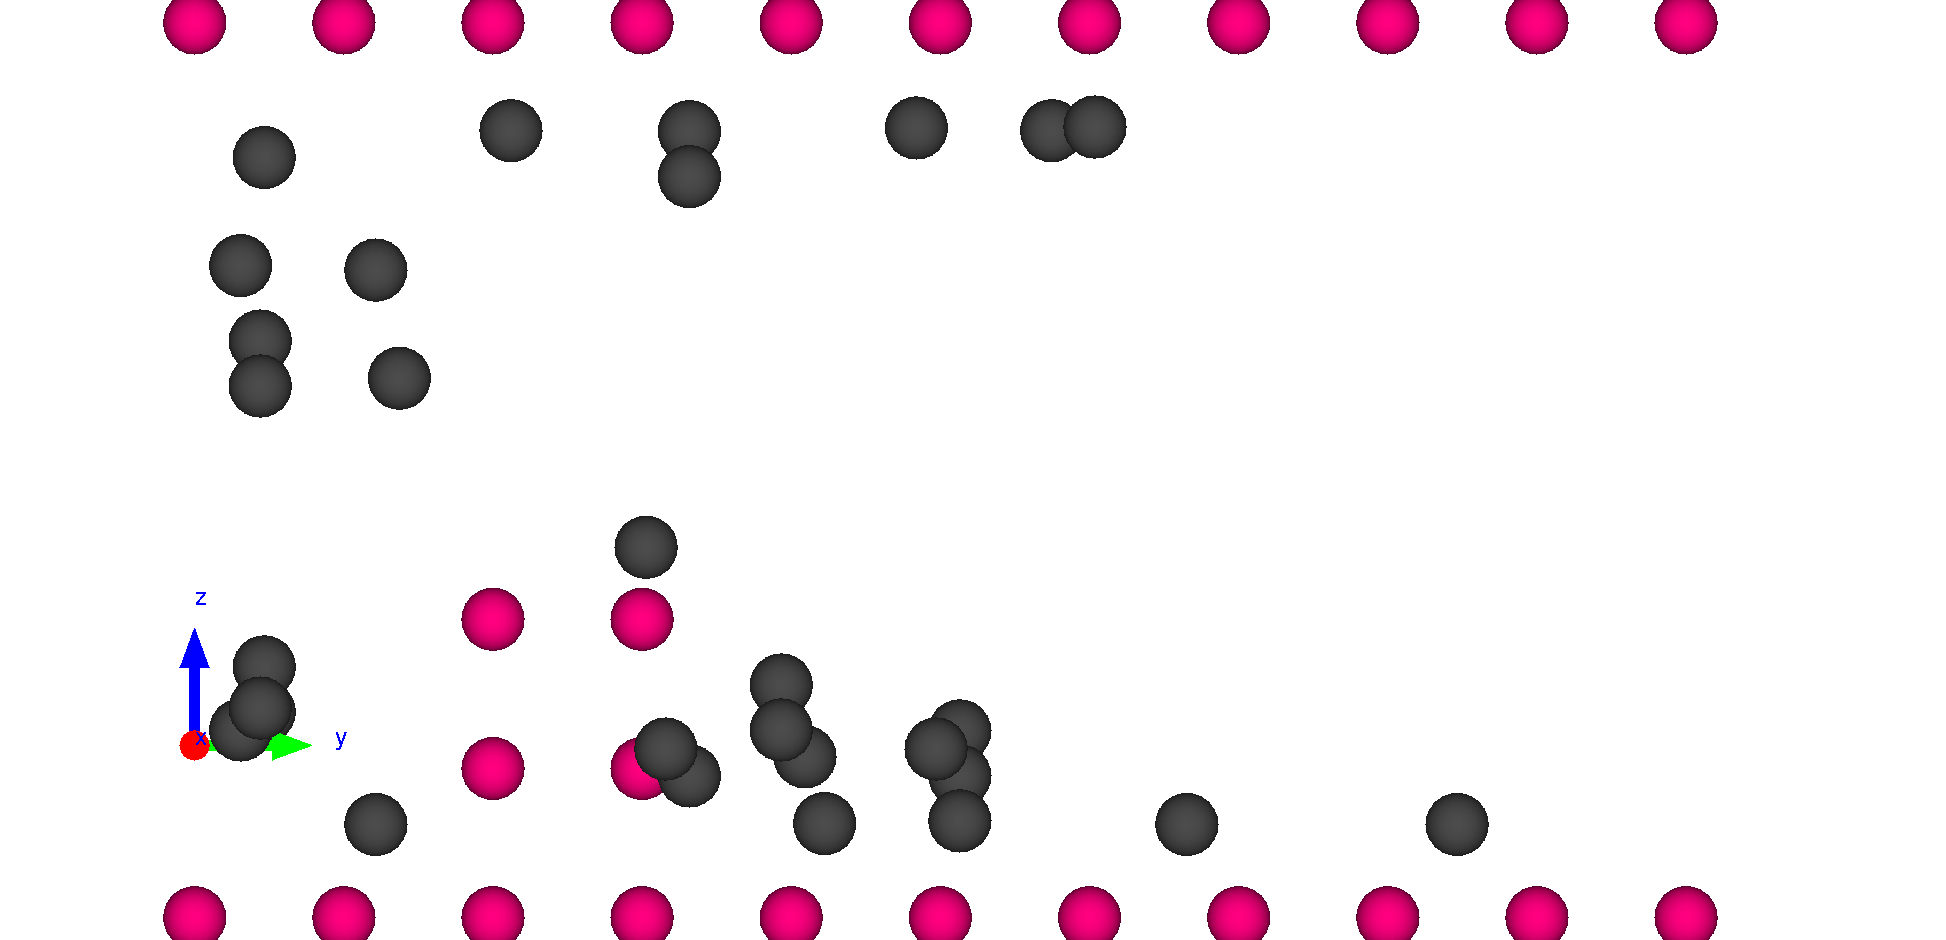
\includegraphics[height=50px]{img/390.pdf}
    \caption{Разрушение филамента в процессе RESET после 3900 шагов КМК
    }
\end{figure}
\end{multicols}
\end{frame}

%Есть надежда получить реакции set-reset и показать их оттельно, но пока еще нет.
\begin{frame}{ВАХ смоделированной системы}
    Была проведена симуляция системы при разных напряжениях и начальных условиях.
    Это позволило получить Вольт-амперную характеристику.
        \begin{figure}
            \centering
            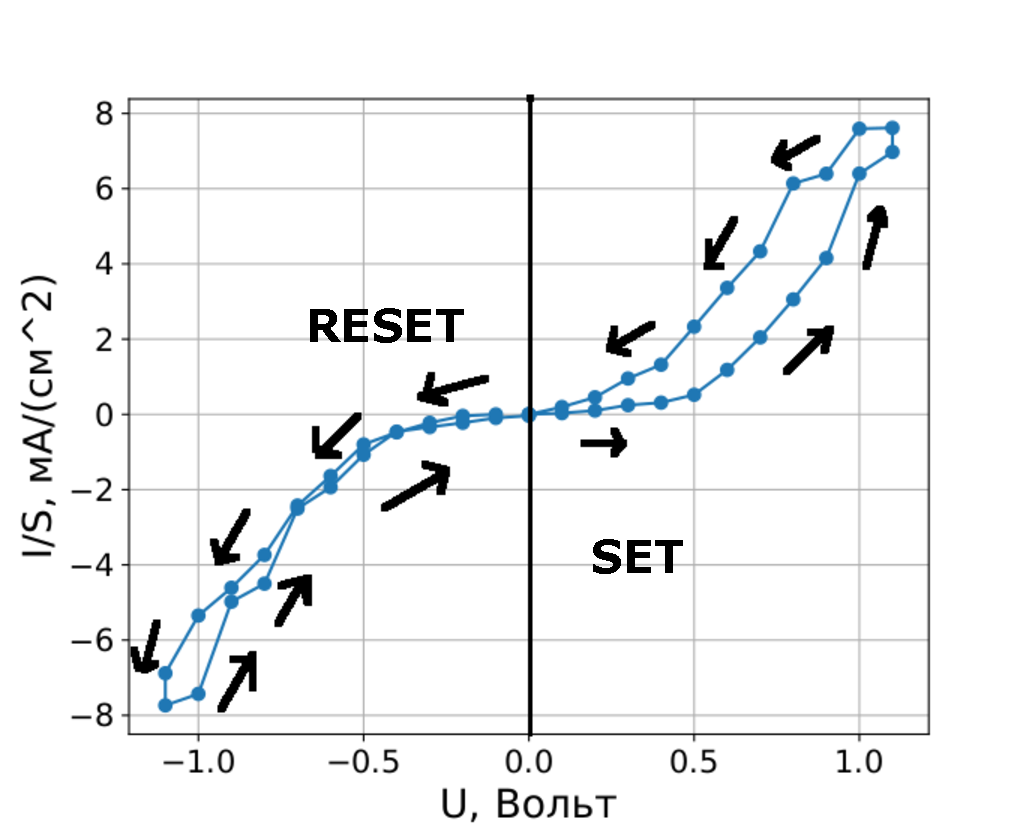
\includegraphics[width=200px]{img/VAH_omg_ex.pdf}
            \caption {Процессы SET-RESET}
        \end{figure}

\end{frame}

%Слайд с обобщенными результатами
\begin{frame}{Результаты}

\begin{list}{*}{}
    \item  Разработана и реализована модель для симуляции роста филаментарных структур с использованием кинетического метода Монте-Карло
    \item  С использование теории функционала плотности выполнены рассчеты для параметризации процессов.
    \item  Работа модели была проверена, и на её основании было получены и продемонстрировано образование филаментарной структуры при наличии внешнего поля.
\end{list}
\end{frame}
%Слайд с тем, что еще можно сделать
\begin{frame}{Планы}

\begin{list}{*}{}
    \item  Учет сложной структуры интерфейса на границе Оксид-Электрод
    \item  Рассмотрение разных форм электрода.
    \item  Рассмотрение разных веществ в качестве электрода/диэлектрика.
    \item  Изучение вклада от разных способов течения тока в общий ток.
\end{list}



\end{frame}

\begin{frame}[plain]
\vfill
\centerline{Спасибо за внимание!}
\vfill\vfill
\end{frame}

%Секретный слайд
%Секретный - потому, что пока показывать во время основной презентации не планирую
\begin{frame}{Set-Reset в мемристоре}
    \begin{figure}
        \centering
        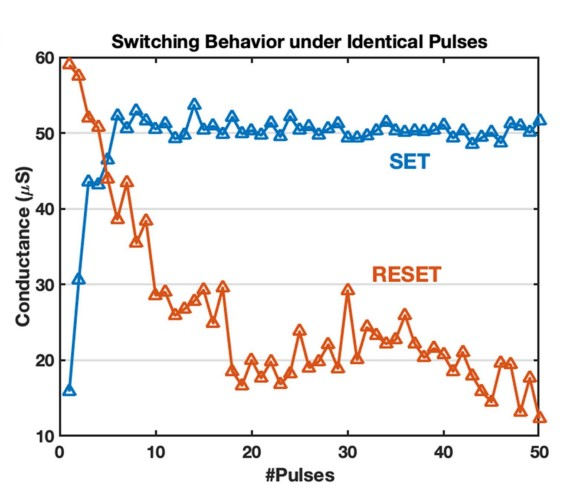
\includegraphics[width=180px]{img/memristor-set-reset.jpg}
        \caption{Set-reset в мемристоре%
    \footnote{%
    Guo Y, Wu H, Gao B and Qian H(2019) Unsupervised Learning on Resistive Memory Array Based Spiking Neural Networks. Front. Neurosci. 13:812. doi: 10.3389/fnins.2019.00812
    }%
  }
    \end{figure}
\end{frame}


\end{document}